\begin{block}{Outlook - the optical vernier}
  Our group developed compact frequency standards for two differen 2-photon Cs transitions (8S at 822 nm and 6D at 884 nm).
  \begin{columns}
    \begin{column}{0.60\textwidth}
     \begin{itemize}
     \item Extended cavity diode laser with intracavity cesium cell
     \item Focused beam for $\approx$ 1000 SNR for 822 nm
     \item Total length of 17 cm
     \end{itemize}
    \end{column}
    \begin{column}{0.39\textwidth}
      \begin{figure}
        \begin{center}
          \includegraphics[width=0.9\textwidth]{figures/compactreference}
        \end{center}
      \end{figure}
    \end{column}
  \end{columns}
  \begin{columns}
    \begin{column}{0.60\textwidth}
     \begin{itemize}
     \item   Combine this with a frequency comb to get an optical vernier.
       \begin{itemize}
       \item 822 nm reference locks the repetition rate
       \item 884 nm reference lock the absolute frequency
       \item CPT transition provides monitoring of the repetition rate, connecting the microwave and optical regime
       \end{itemize}
     \end{itemize}
    \end{column}
    \begin{column}{0.39\textwidth}
      \begin{figure}
        \begin{center}
          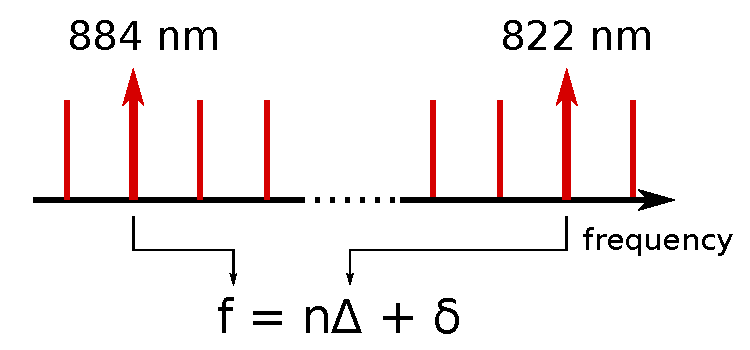
\includegraphics[width=1.0\textwidth]{figures/vernier}
        \end{center}
      \end{figure}
    \end{column}
  \end{columns}
  This scheme removes the need of a highly stable synthetizer, which is an obstacle to a compact and robust design.
\end{block}
